\section{Auswertung}
\label{sec:Auswertung}




  \subsection{Eichung des Elektromagneten}
  In Tabelle \ref{tab:mit} sind die eingestellten Stromstärken $I$ und die mit einer Hallsonde gemessenen zugehörigen Magnetfeldstärken $B$ aufgelistet.
  
  \begin{table}[H] 
	\centering
	\caption{Für die Eichung des Magneten aufgenommene Messwerte des Magnetfeldes neben der zugehörigen Stromstärke} 
	\begin{tabular}{c|c}

Strom I / A & Magnetische Flussdichte B \\ 
\hline 
1	& 60 \\
2	& 123 \\
4	& 236\\
6	& 330\\
8	& 460\\
10	& 580\\
12	& 700\\
14	& 800\\
16	& 890\\
18	& 960\\
20	& 1020\\	
		
	\end{tabular} 
	  \label{tab:mit}
\end{table} 

\begin{figure}[h]
	\centering
	\includegraphics[width=12cm,height=8cm]{plot/V27_plot_1.pdf}
	\caption{Magnetischer Flussdichte gegen Stromstärke aufgetragen}
	\label{plot:1}
\end{figure}

Mit den Messwerten aus Tabelle \ref{tab:mit} wird eine Ausgleichsrechnung mittels der Funktion 
\begin{align}
f(x)= ax+b
\end{align}

durchgeführt. Für die Parameter erhält man durch den Fit:

\begin{center}
a = 52,4581 \pm 1,512 $\frac{mT}{A}$
\\
b = 30,5592 \pm 17,9 $mT$

\end{center}    



  \subsection{\texorpdfstring{Aufl"oseverm"ogen $A$ und Dispersionsgebiet $\Delta \lambda$ der verwendeten Lummer-Gehrcke-Platte f"ur die Wellenl"angen des roten und blauen "Ubergangs}{Aufl"oseverm"ogen A und Dispersionsgebiet Delta lambda der verwendeten Lummer-Gehrcke-Platte f"ur die Wellenl"angen des roten und blauen "Ubergangs}}
  
  Die zur Berechnung notwendigen Größen sind in der Versuchsanleitung gegeben
  
  \begin{center}
  L = 120 mm \\
  d = 4 m \\
  n(644nm) = 1,4567 \\
  n(480nm) = 1,4635. \\
  \end{center}
Das Dispersionsgebiet $\Delta \lambda$ und das Auflösevermögen $A$ wurden mit den folgenden Formeln berechnet und in der Tabelle aufgeführt.
  \begin{equation}
\Delta \lambda_D=\frac{\lambda^2}{2d}\cdot \sqrt{\frac{1}{n^2-1}}
\end{equation}

\begin{equation}
A=\frac{\lambda}{\Delta = \lambda}\frac{L}{\lambda}\Bigl(n^2-1\Bigr)
\end{equation}

  
    \begin{table}[H] 
	\centering
	\caption{Dispersionsgebiet $\Delta \lambda$ und das Auflösevermögen $A$} 
	\begin{tabular}{c|c|c}

  & rot & blau\\ 
\hline 
$\lambda$	 		& 643,8 nm & 480 nm \\
$\Delta \lambda $	& 48,91 pm & 26,95 pm \\
A				& 209129 & 285458 \\

		
	\end{tabular} 
	  \label{tab:mit2}
\end{table} 
  \newpage
    \subsection{\texorpdfstring{Bestimmung des Lande-Faktors $g_{12}$ der $\sigma$-"Uberg"ange f"ur die rote Linie}{Bestimmung des Lande-Faktors g_{12} der sigma-"Uberg"ange f"ur die rote Linie}}
    
    Für die rote Spektrallinie der Wellenlänge $\lambda = 643.8 nm$ wurden folgende Bilder aufgenommen werden
    
    \begin{figure}[h]
	\centering
	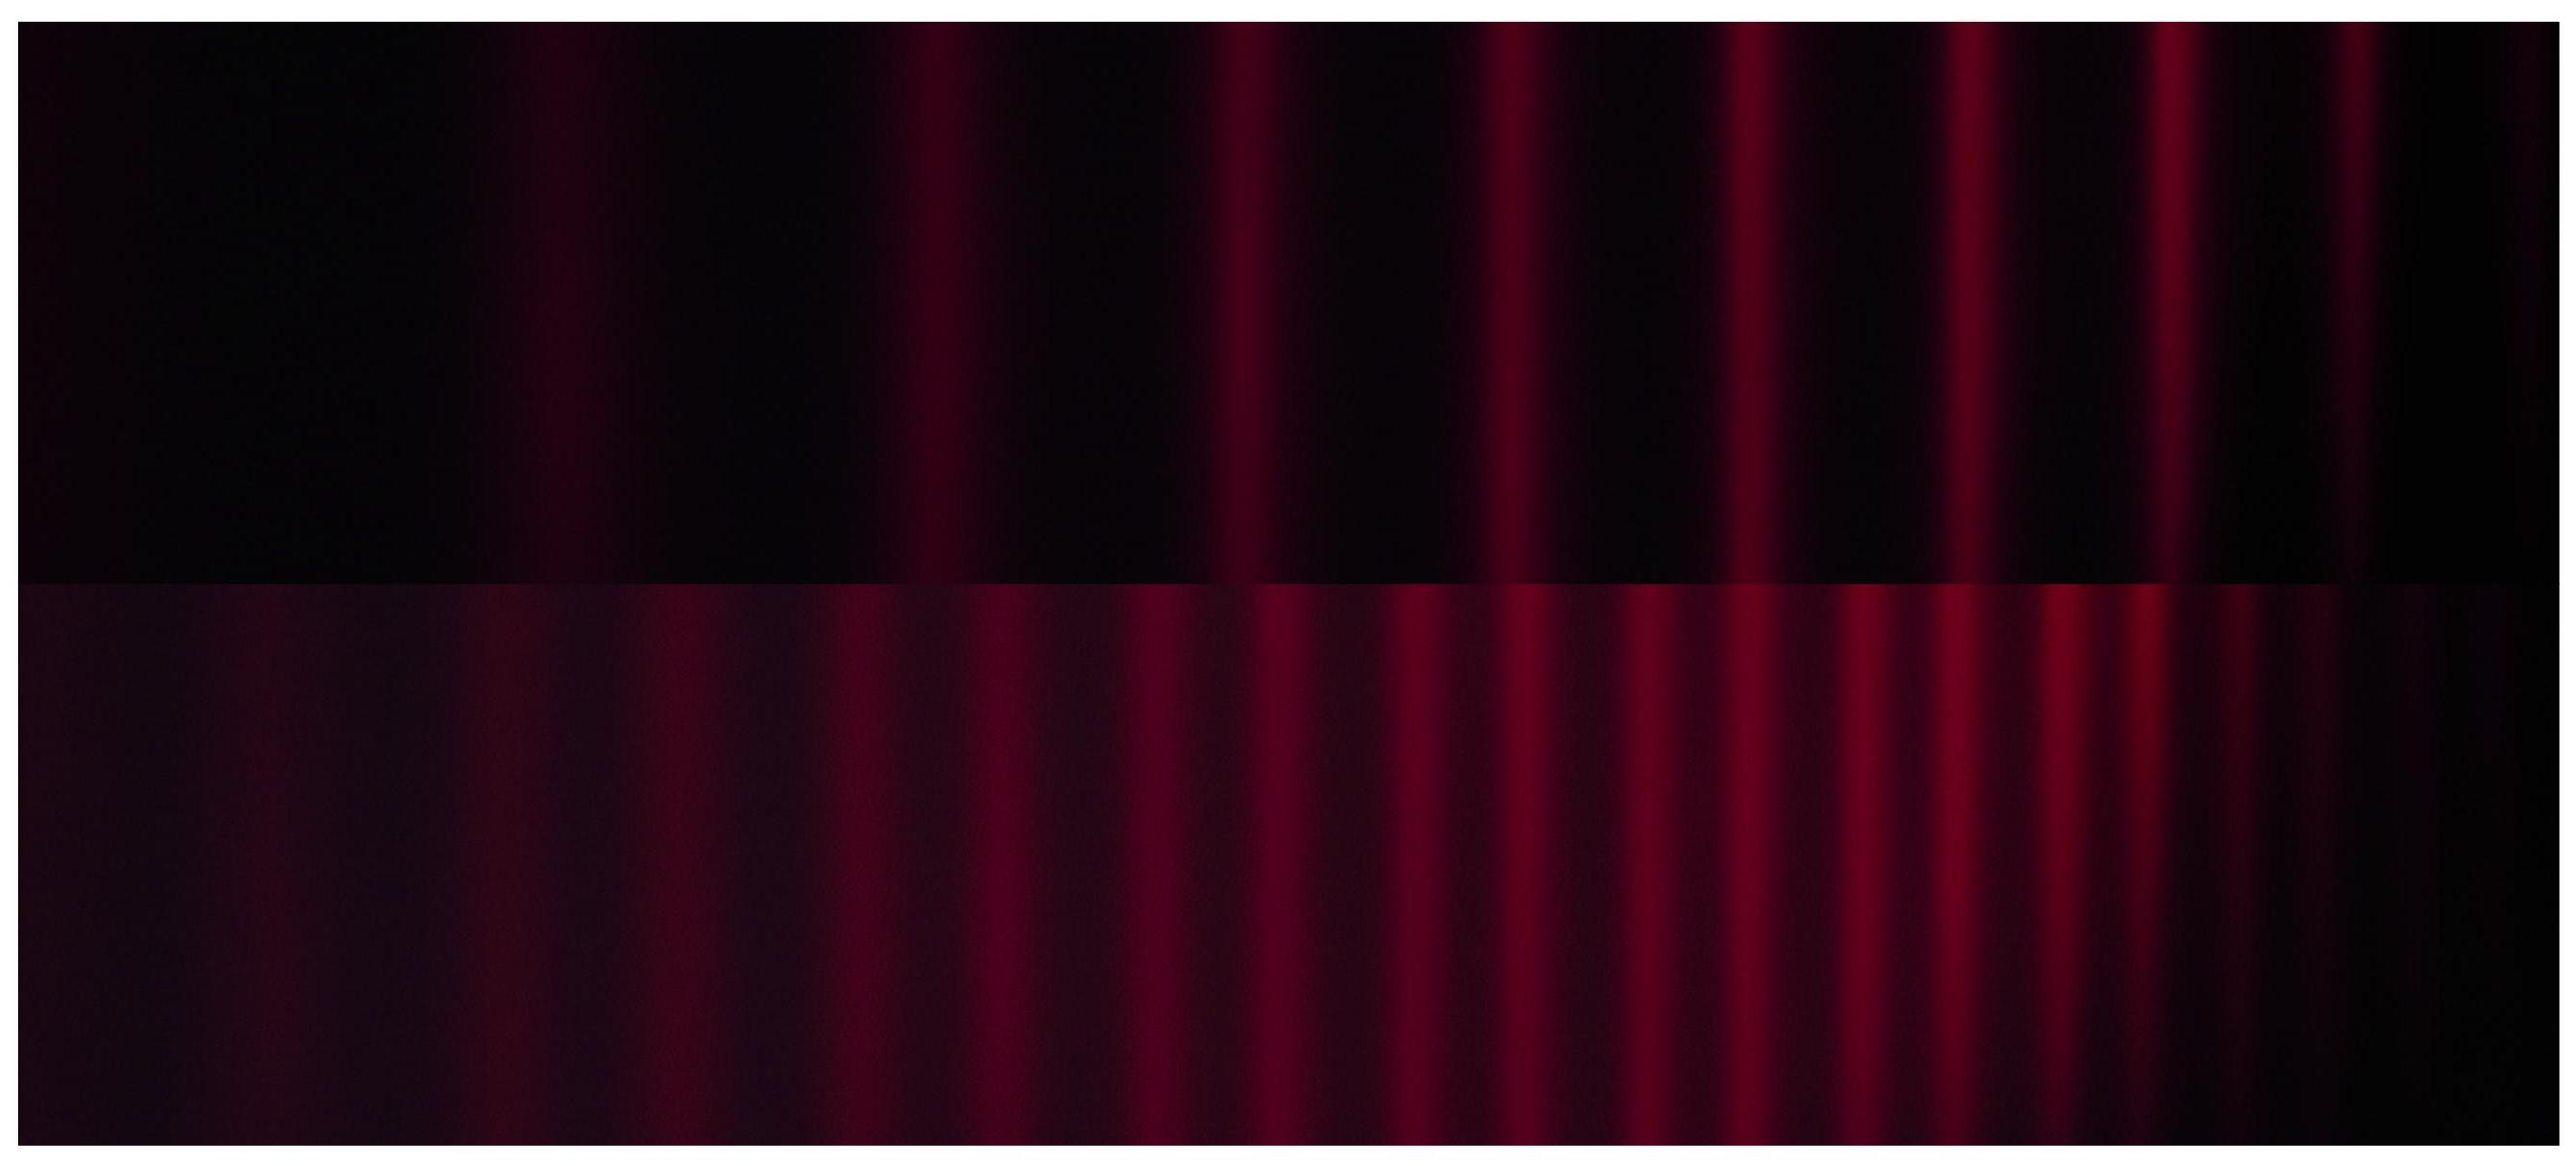
\includegraphics[width=16cm,height=6cm]{Fotos/V27_1.jpg}
	\caption{Interferenzmuster bei Rot (oben B=0, unten B=605 mT)}
	\label{plot:1}
\end{figure}
    
 Dabei entspricht das obere Muster dem Interferenzmuster bei ausgeschaltetem Magnetfeld (B=0) und das untere Muster den Interferenzmuster bei eingeschaltetem Magnetfeld (B=605 mT). Aus diesen Interferenzmustern wurden mittels Vorschau die in Tabelle \ref{tab:mit3} aufgelisteten Werte ermittelt. Die Wellenlängenverschiebung wurde dabei mittels folgender Formel berechnet:
    
    \begin{equation}
  \label{gl:gleichung}
  \delta\lambda=\frac{\delta s}{2\Delta s} \cdot \Delta\lambda_D
\end{equation}

  \begin{table}[H] 
	\centering
	\caption{Messwerte zur Bestimmung der Wellenlängenänderung} 
	\begin{tabular}{c|c|c|c}

  & $\Delta$ s in px & $\delta s$ in px & $\delta \lambda$ in $10^{-12} m$\\
  \hline 
1 &479&214&10,92 \pm 0,17 \\
2 &339&148&10,68 \pm 0,24 \\
3 &276&131&11,61 \pm0,29 \\
4 &238&104&10,69 \pm0,34 \\
5 &215&95&10,81 \pm 0,37 \\
6 &198&75&9,26 \pm 0,40 \\
7 &174&64&8,99 \pm 0,45 \\
8 &157&60&9,35 \pm 0,50 \\

		
	\end{tabular} 
	  \label{tab:mit3}
\end{table} 

Werden die berechneten Werte gemittelt, ergibt sich für die Wellenlängenverschiebung:

\begin{center}
$\delta \lambda$ = (10,29 \pm 0,21) pm
\end{center}

  \subsection{\texorpdfstring{Bestimmung des Lande-Faktors $g_{12}$ der $\pi$-"Uberg"ange f"ur die blaue Linie}{Bestimmung des Lande-Faktors g_12 der pi-"Uberg"ange f"ur die blaue Linie}}
  
Bestimmung des Lande-Faktors $g_{12}$ der $pi$-Übergänge für die blaue Linie wird nach dem selben Schema wie im Aufgabenteil 4.4. 
  
        \begin{table}[H] 
	\centering
	\caption{Messwerte zur Bestimmung der Wellenlängenänderung} 
	\begin{tabular}{c|c|c|c}

  & $\Delta$ s in px & $\delta s$ in px & $\delta \lambda$ in $10^{-12} m$\\
  \hline 
1&188&92&6,59 \pm 0,24 \\
2&176&84&6,43 \pm 0,25 \\
3&160&72&6,06 \pm 0,28 \\
4&147&63&5,77 \pm 0,30 \\
5&131&58&5,97 \pm 0,34 \\
6&122&52&5,74 \pm 0,36 \\

		
	\end{tabular} 
	  \label{tab:mit4}
\end{table} 

\begin{figure}[h]
	\centering
	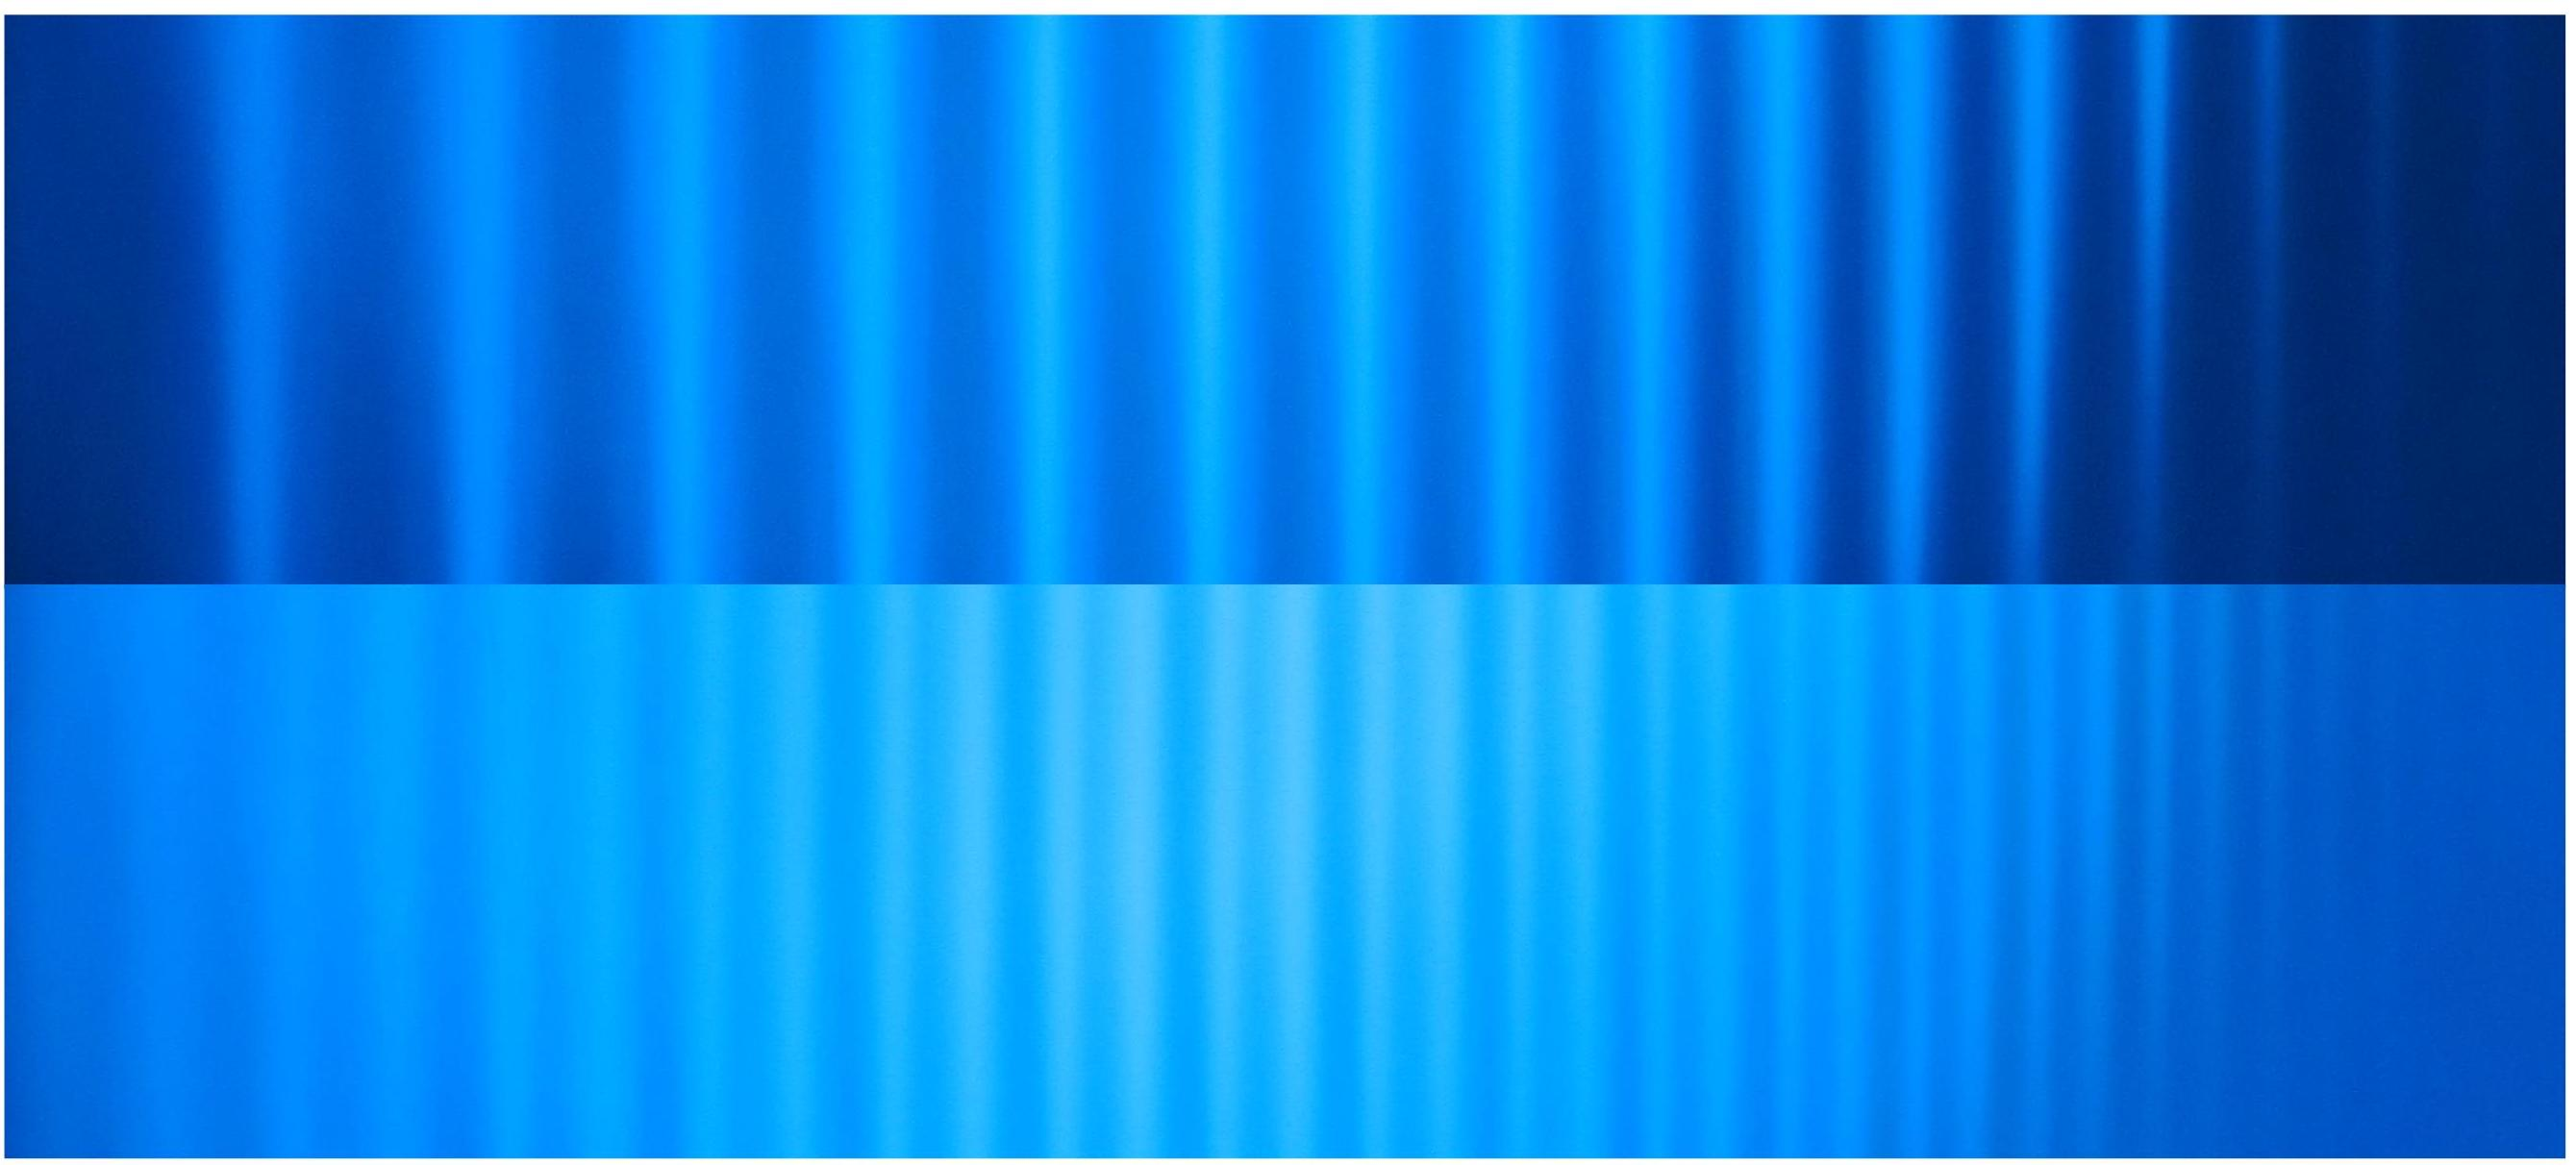
\includegraphics[width=16cm,height=6cm]{Fotos/V27_2.jpg}
	\caption{Interferenzmuster bei Blau (oben B=0, unten B=360 mT)}
	\label{plot:1}
\end{figure}

\begin{center}
$\delta \lambda$ = (6,09 \pm 0,22) pm
\end{center}

\newpage

  \subsection{\texorpdfstring{Bestimmung des Lande-Faktors $g_{12}$ der $\sigma$-"Uberg"ange f"ur die blaue Linie}{Bestimmung des Lande-Faktors g_{12} der sigma-"Uberg"ange f"ur die blaue Linie}}
  
  Bestimmung des Lande-Faktors $g_{12}$ der $sigma$-Übergänge für die blaue Linie wird nach dem selben Schema wie im Aufgabenteil 4.4. 
  
          \begin{table}[H] 
	\centering
	\caption{Messwerte zur Bestimmung der Wellenlängenänderung} 
	\begin{tabular}{c|c|c|c}

  & $\Delta$ s in px & $\delta s$ in px & $\delta \lambda$ in $10^{-12} m$\\
  \hline 
1&178&90&6,81 \pm 0,25 \\
2&172&86&6,73 \pm 0,26\\
3&160&74&6,23 \pm 0,28\\
4&144&58&5,42 \pm 0,30\\
5&124&53&5,76 \pm 0,35\\
6&118&49&5,59 \pm 0,37\\
7&111&44&5,34 \pm 0,39 \\

		
	\end{tabular} 
	  \label{tab:mit5}
\end{table} 

\begin{figure}[h]
	\centering
	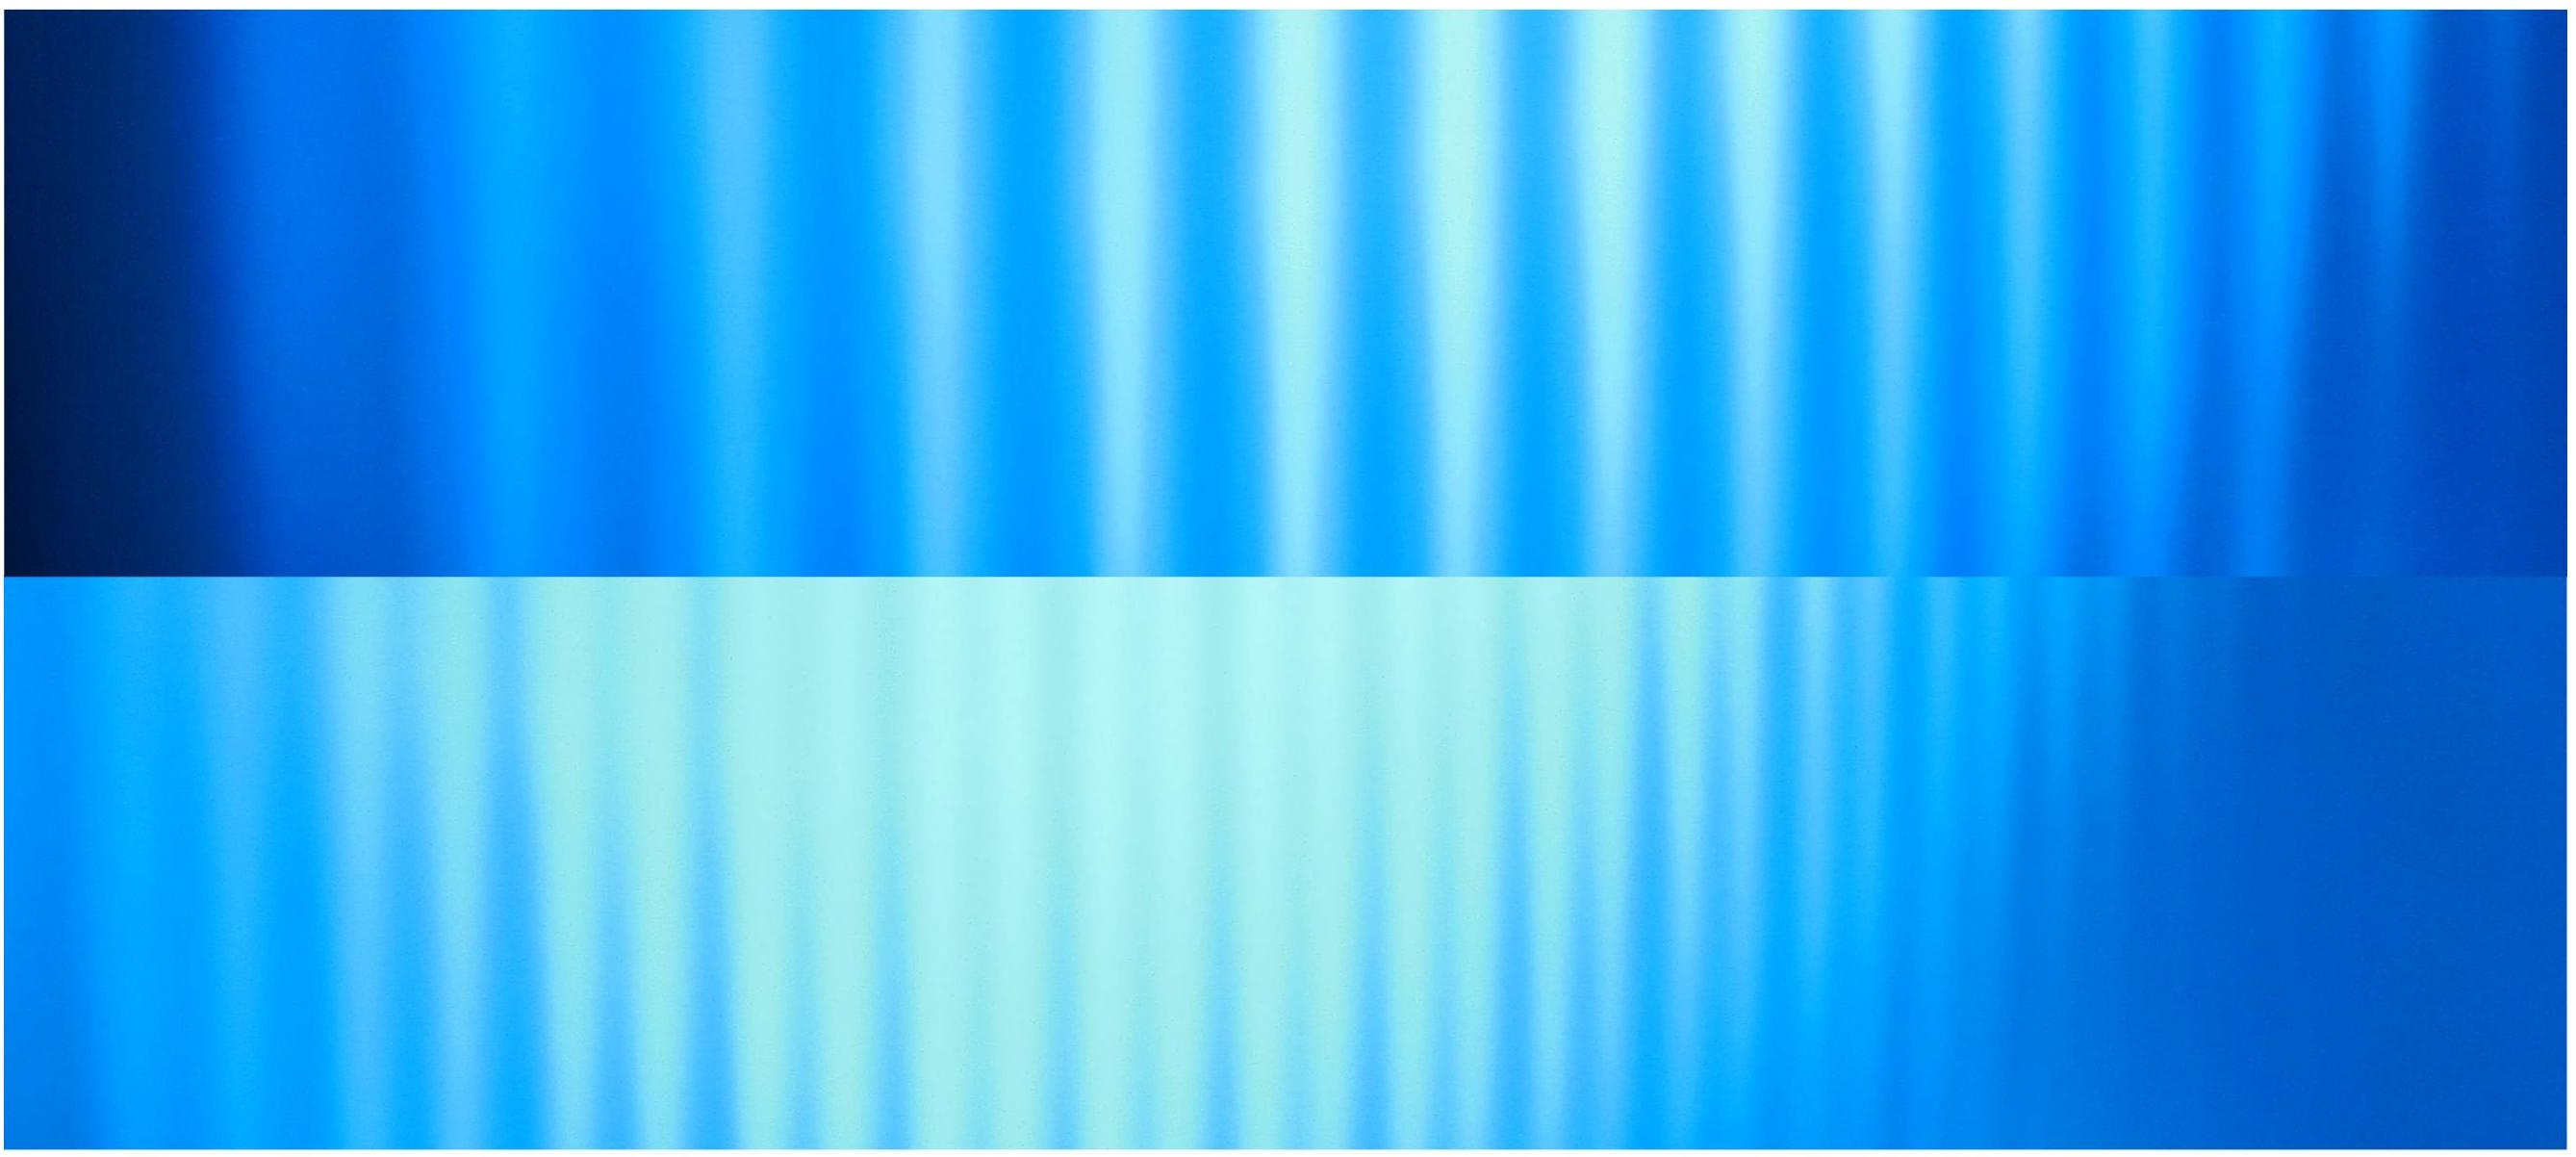
\includegraphics[width=16cm,height=6cm]{Fotos/V27_3.jpg}
	\caption{Interferenzmuster bei Blau (oben B=0, unten B=1020 mT)}
	\label{plot:1}
\end{figure}

\begin{center}
$\delta \lambda$ = (5,99 \pm 0,21) pm
\end{center}


  \subsection{\texorpdfstring{Berechnung der experimentellen Lande-Faktoren $g_{ij}$ aus den Abst"anden $\Delta s$ und $\delta s$ der erhaltenen Aufnahmen}{Berechnung der experimentellen Lande-Faktoren g_{ij} aus den Abst"anden Delta s und delta s der erhaltenen Aufnahmen}}

  $\Delta s$ ist der Abstand der benachbarten Interferentzmaxima in der Aufnahme ohne Magnetfeld, $\delta s$ ist die Breite der Aufspaltung eines Interferenzmaximas, in der Aufnahme mit angelegtem Magnetfeld mit St"arke $B$.
  Damit ergibt sich f"ur den Wellenl"angenunterschied $\delta \lambda$ zwischen den beiden Energieniveaus des "Ubergangs
  \begin{equation}
    \delta \lambda = \frac{1}{2}\frac{\delta s}{\Delta s} \Delta \lambda \; .
  \end{equation}
  Mit
  \begin{align}
    \begin{split}
    \frac{\partial E}{\partial \lambda} = \frac{\delta E}{\delta \lambda} &= \frac{\delta}{\delta \lambda} \frac{hc}{\lambda} = -\frac{hc}{\lambda^2}\\
    \iff \delta E &= \frac{ch}{\lambda^2} \delta \lambda
   \end{split}
  \end{align}
  folgt f"ur den Lande-faktor $g_{12}$ mit der Energieniveaudifferenz $\delta E$/Wellenl"angendifferenz $\delta \lambda$ nach Formel (\ref{g_ij}) der Zusammenhang
  \begin{equation}
    g_{12}=\frac{\delta E}{\mu_BB}=\frac{hc\delta \lambda}{\lambda^2\mu_BB} \; .
  \end{equation}

          \begin{table}[H] 
	\centering
	\caption{Für die Eichung des Magneten aufgenommene Messwerte des Magnetfeldes neben der zugehörigen Stromstärke} 
	\begin{tabular}{c|c|c|c|c}

  $\lambda$ pm & B mT & Übergang & $g_{ij,exp}$& $g_{ij,theo}$\\
  \hline 
643,8 & 632 &$\sigma$&0,84&1\\
480 &360&$\sigma$&1,55&1,25\\
480 &1020 &$\pi$&0,55&0,5\\


		
	\end{tabular} 
	  \label{tab:mit6}
\end{table} 



















